% Use only LaTeX2e, calling the article.cls class and 12-point type.

\documentclass[12pt]{article}

% Users of the {thebibliography} environment or BibTeX should use the
% scicite.sty package, downloadable from *Science* at
% www.sciencemag.org/about/authors/prep/TeX_help/ .
% This package should properly format in-text
% reference calls and reference-list numbers.

\usepackage{scicite}

% Use times if you have the font installed; otherwise, comment out the
% following line.

\usepackage{times}
\usepackage{graphicx}
\usepackage{listings}
\usepackage [table]{xcolor  }

\newenvironment{code}{\begin{tabbing}
12345\=12345\=12345\=12345\=12345\=12345\=12345\=12345\= \kill }
{\end{tabbing}}

% The preamble here sets up a lot of new/revised commands and
% environments.  It's annoying, but please do *not* try to strip these
% out into a separate .sty file (which could lead to the loss of some
% information when we convert the file to other formats).  Instead, keep
% them in the preamble of your main LaTeX source file.


% The following parameters seem to provide a reasonable page setup.

\topmargin 0.0cm
\oddsidemargin 0.2cm
\textwidth 16cm 
\textheight 21cm
\footskip 1.0cm


%The next command sets up an environment for the abstract to your paper.

\newenvironment{sciabstract}{%
\begin{quote} \bf}
{\end{quote}}


% If your reference list includes text notes as well as references,
% include the following line; otherwise, comment it out.

\renewcommand\refname{References and Notes}

% The following lines set up an environment for the last note in the
% reference list, which commonly includes acknowledgments of funding,
% help, etc.  It's intended for users of BibTeX or the {thebibliography}
% environment.  Users who are hand-coding their references at the end
% using a list environment such as {enumerate} can simply add another
% item at the end, and it will be numbered automatically.

\newcounter{lastnote}
\newenvironment{scilastnote}{%
\setcounter{lastnote}{\value{enumiv}}%
\addtocounter{lastnote}{+1}%
\begin{list}%
{\arabic{lastnote}.}
{\setlength{\leftmargin}{.22in}}
{\setlength{\labelsep}{.5em}}}
{\end{list}}


% Include your paper's title here

\title{Identifying Reproducibility in Scientific Publications} 


% Place the author information here.  Please hand-code the contact
% information and notecalls; do *not* use \footnote commands.  Let the
% author contact information appear immediately below the author names
% as shown.  We would also prefer that you don't change the type-size
% settings shown here.

\author
{Text as Data: Final Project \\
\\
Al\'i J. Lim\'on, Felipe N. Ducau\\
\normalsize{New York University}\\
}

% Include the date command, but leave its argument blank.

\date{}



%%%%%%%%%%%%%%%%% END OF PREAMBLE %%%%%%%%%%%%%%%%



\begin{document} 

% Double-space the manuscript.

\baselineskip24pt

% Make the title.

\maketitle 



% Place your abstract within the special {sciabstract} environment.

\begin{sciabstract}
  Ideally all scientific studies should be reproducible and verified by other researchers before publication. However, because of strong incentives for innovation and weak incentives for confirmation, direct replication is rarely practiced or published. In the scientific world there is a growing alarm not only because of lack of replications, but also because it was noted that an important amount of scientific publications are not replicable.  Our project consists on analyze publications for which we know if there was a successful replication or not, and train a machine learning classifier with text features from aforementioned papers with the goal of predicting if the results presented in a new unobserved publication are actually valid or not. 
\end{sciabstract}



% In setting up this template for *Science* papers, we've used both
% the \section* command and the \paragraph* command for topical
% divisions.  Which you use will of course depend on the type of paper
% you're writing.  Review Articles tend to have displayed headings, for
% which \section* is more appropriate; Research Articles, when they have
% formal topical divisions at all, tend to signal them with bold text
% that runs into the paragraph, for which \paragraph* is the right
% choice.  Either way, use the asterisk (*) modifier, as shown, to
% suppress numbering.

\section{Introduction}
\quad \textbf{Scenario} 

The power of science rests on the assumption that results are replicable, and that high standards are maintained by anonymous peer review. This is what allows new results to be built on top of earliest research and discoveries. In September 2015, the international scientific journal Nature \cite{nature1} published a cartoon showing the temple of “Robust Science” in a state of collapse. 
The replicability of several scientific findings has recently been called into question. According to the mentioned Nature article,  an unpublished 2015 survey by the American Society for Cell Biology found that more than two-thirds of respondents had on at least one occasion been unable to reproduce published results. Furthermore, biomedical researchers from drug companies have reported that one-quarter or fewer of high-profile papers are reproducible \cite{begley, prinz}.

In order to address this problem, experimental researchers have joined the reproducibility discussion by replicating selected published experiments from two top-tier journals in economics, biology and psychology.

\textbf{Hypothesis}

In this project we analyze if it is possible to determine if a scientific publication contains within its text some information about its replicability. Our hypothesis is that there is sufficient information embedded in the body of a published paper to recognize if the reported results are reproducible or not. Our question is, do scientist write in a different way when they are presenting flawed or false results? The way the results are presented, the language used and the level of obfuscation when presenting results might lead us to determine the reproducibility of the research.


\textbf{Previous Work}

Prior work has evaluated the writing style of a single fraudulent author, social psychologist Diederik Stapel, finding that his writing style differed across his fraudulent and genuine papers \cite{prev}. In \cite{prev2}, the same authors look for linguistic patterns in fraudulent publications, yielding a 57\% accuracy in classifying fraudulent from non-fraudulent publications. They based most of their work in evaluating how obscure is the language used in those papers and create a very simple obfuscation index based in jargon use, an abstraction index, use of positive motion terms and casual terms and FRE score.

\textbf{Source Code}

All the code, and datasets used for this project along with a copy of this work can be found in the GitHub repository \texttt{https://github.com/fnd212/TAD\_Project\_2016.git}.


\section{Data} 

Our labeled data comes from The Reproducibility Project \cite{rep_proj}, by the Center for Open Science. The project is an open, large-scale, collaborative effort to systematically examine the rate and predictors of reproducibility in psychological science. Their original project conducted replications of 100 experimental and correlational studies published in three psychology journals using, when possible, original materials. From these 100 papers, 97 reported P values lower than 0.05, after replicating this studies, only 39 still got significant results, leading to 61 confirmed unreplicable studies. Figure \ref{fig:replication} shows an schematic of the results reported by the study. 

From the results published \footnote{https://osf.io/fgjvw/} we extracted the names of the papers, the authors and the ``Replicated'' colum which has a boolean value that indicates wether the results of the original paper where successfully replicated or not. Afterwards we downloaded the PDF files of the papers from the dataset and used the text in them for our analysis. Because the results of the Reproducibility Project had two duplicated entries and we could not have access to one of the papers, we end up with 97 papers to analyze from which 31 are labeled as reproducible and 61 as unreproducible.

\begin{figure}[htbp]
    \centering
    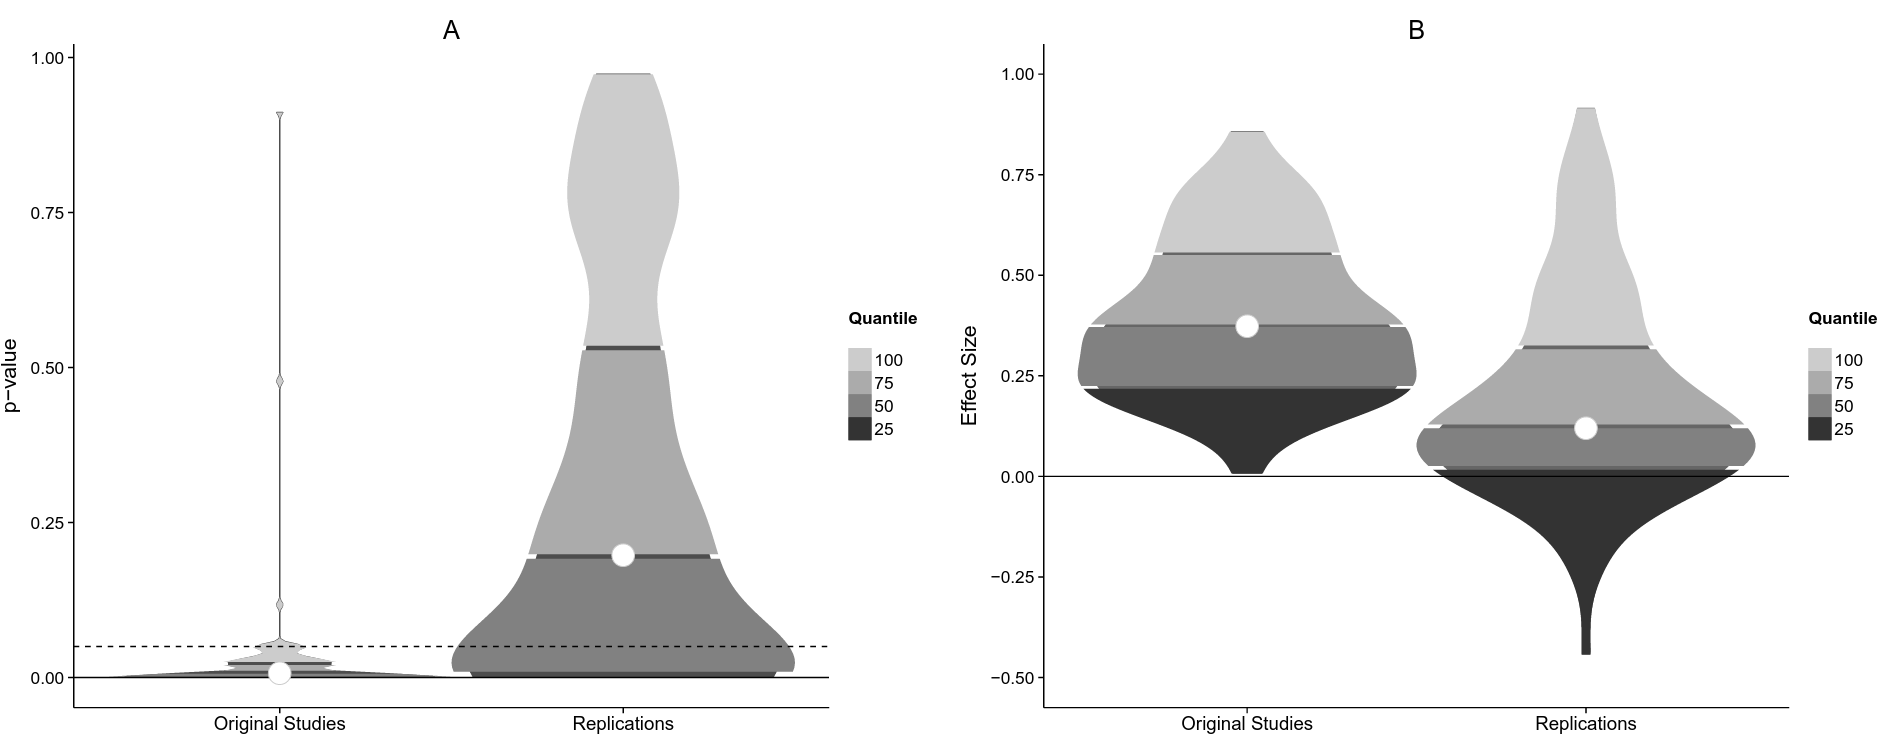
\includegraphics[width=1\textwidth]{dataset_structure}
    \caption{Reproducibility Project results (Source: https://osf.io/7js8c/). A shows the distribution of the p-values reported in the original studies and in the replications. B shows the effect size in both cases.}
    \label{fig:replication}
\end{figure}

Since the major difficulty for our project is the limited amount of labeled data we have to carry our analysis, and given the fact that the two classes in which we classify the publications  (reproducible and not reproducible) are unbalanced, we decided to collect 21 extra papers, with the intention to increase the number of observations for our dataset one the one hand, and to balance the classes on the other. Since, as already mentioned, it is not trivial to determine if a paper is replicable or not beforehand, we make the assumption that, if an author has published a paper that was replicated successfully, then the rest of his/her work is also replicable. Therefore all the 21 new papers belog to the replicable class and belongs to authors which are already present in the dataset and labeled as replicable as well. 

\begin{figure}[htbp]
    \centering
    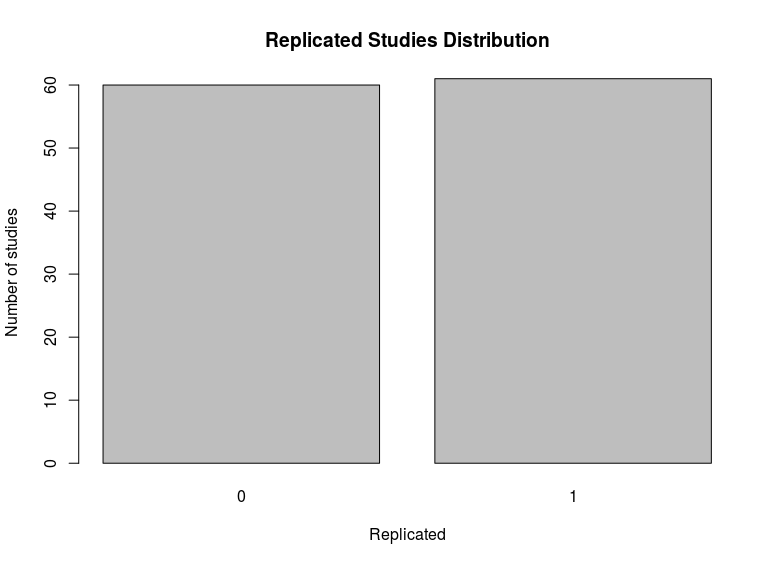
\includegraphics[width=0.6\textwidth]{ds_exploration_01}
    \caption{Classes distribution in the final dataset. Class 1 belongs to replicated papers while class 0 refers tu unreplicable papers.}
    \label{fig:classes}
\end{figure}

\textbf{Preprocessing}

The first task we performed on the paper files was to convert them into txt. For this purpose we used two different methods: (1) we used the Linux software \texttt{pdftotext v3.03}  \footnote{The pdftotext software and documentation are copyright 1996-2004 Glyph \& Cog, LLC.}, unfortunately the output of this tool is still very noisy and has problems identifying objects such as tables or equations. We generated a second version for each paper with \texttt{pdfx1.9}\footnote{http://pdfx.cs.man.ac.uk/}, a tool optimized to convert text from scientific articles to xml \cite{pdfx} which afterwards we parsed with an R script to get the txt file. Further preprocessing steps were applied according to the requirements of each of the models we used and will be explained within the corresponding model section. 



\section{Methodology}

Because of the nature of the data we decided to take two different approaches for the classification task. The first one, using a sparse representation of the text, uses bag of words and tf-idf to train machine learning models. The second approach is intended to use condensed features, and makes use of aggregated indices computed from the text using the LIWC dictionary and other characteristics of the text we consider relevant. Once we computed all the indices we applied multiple machine learning models in order to predict the target variable. As the characteristics of the features between models is different,  we apply specific preprocessing and machine learning tools for each approach to extract as much information as possible from this classifiers. 

Because of the size of our dataset, it could be misleading to do a train/test sample, perform cross-validation (for those classifiers that applies) on the train set and evaluate the performance on the test set. The performance metrics we would obtain by this approach would be highly dependant on the random split, and different random splits can lead to fairly different results. Instead of these, we decided to evaluate our ``procedure'' instead of evaluating a particular model performance. 

Our approach consists on doing $n$ train/test different random splits of the data, train (and cross-validate the hyperparameters when applicable) the model in each train split and evaluate its performance in the corresponding test split. With this results we then compute the mean accuracy of the classifiers along with its standard deviation, and those are the values to be reported. The idea behind this methodology is that, if we had enough data to do the standard approach, our results would be still accurate with certain degree of statistical confidence. 

The machine learning models are trained with 90 percent of the sample and tested with the other 10 percent. For those models that requires tuning of hyperparameters 10-fold cross-validation was used. The following pseudocode illustrates this procedure. Here the fit method of ``Classifier'' performs the cross-validation procedure when applicable. For our work we decided to set $n$ to 100.\\

\begin{lstlisting}
Compute-Classifier-Performance (Classifier, Dataset):
    for i=1 to n: 
        train, test = RandomSplit(Dataset, 0.9,0.1)
        Classifier.fit(train.X, train.Y)
        predictions = Classifier.predict(test.X)
        accuracy[i] = Accuracy(test.Y, predictions)
    return mean(accuracy), std(accuracy)
\end{lstlisting}

Figure \ref{fig:normal} shows the results of this approach for a Ridge classifier using cross-validation to set the regularization parameter. Since the distribution is similar to a normal distribution, we conclude that the use of two standard deviations from the mean is a reasonable approach for our confidence intervals. 

\begin{figure}[htbp]
    \centering
    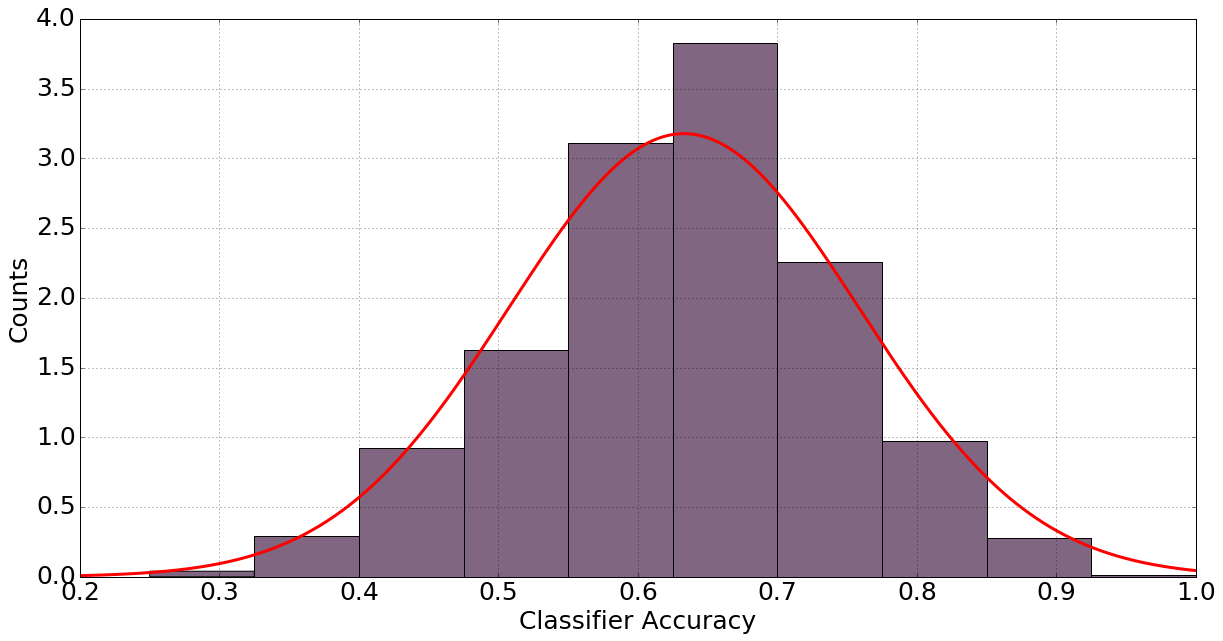
\includegraphics[width=0.8\textwidth]{index}
    \caption{Histogram of accuracy for Ridge classifier.}
    \label{fig:normal}
\end{figure}


\textbf{Sparse Text Representation Approach}

The first step with this approach was to compute the bag-of-words and tf-idf matrices. In order to avoid overfitting as much as possible, we dropped punctuation, stopwords, numbers, and words with less than 3 characters. Additionally, stemming was applied to the words along with lower case conversion to all the text. We used these two matrices to feed a linear SVM modem. Additionaly we also used a Naive Bayes approach to classify the text using the DFM representation of the text.

The results of these approaches are visualized in Figure \ref{fig:bow_model} for the best text representation of each case. The full comparative results of all the models is presented Appendix B. 

\begin{figure}[htbp]
    \centering
    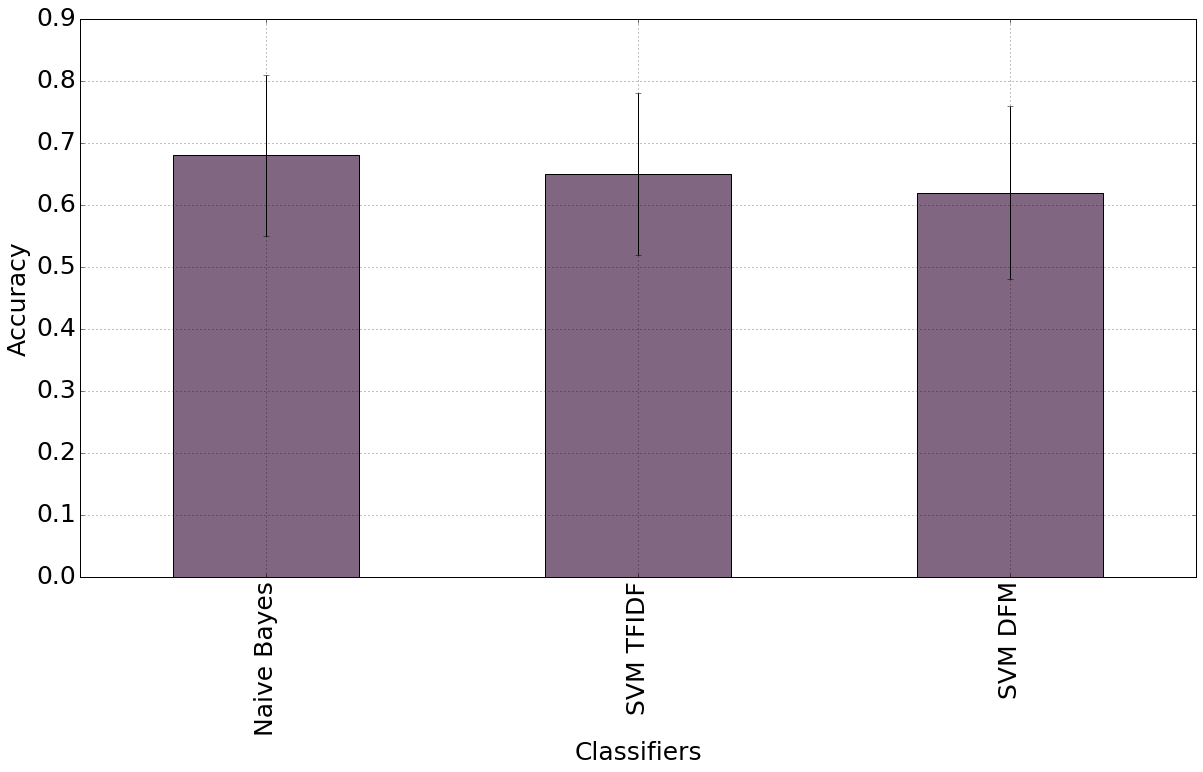
\includegraphics[width=0.9\textwidth]{barplot_words_classifiers}
    \caption{Accuracy performance for sparse text representation approaches.}
    \label{fig:bow_model}
\end{figure}

The accuracies obtained by these models is surprisingly high, so we decide to look at the top 5 (table \ref{tab:results_1}) words which most contribute to classify a text in each of the classes. Even though this words do not contain much information per-se, we can not discard that the actual performance of these classifiers would be equally high in a larger dataset setup. Furhter evaluation of the applicability of these methods for this kind of task is subject to a deeper evaluation in a setup with more labeled data. 

\begin{center}
\label{tab:results_1}
    \begin{tabular}{c|c}
        Replicate = 1 & Replicate = 0 \\ \hline \hline
        rebel         & balota        \\ 
        forgiv        & attractor     \\ 
        victim        & besner        \\ 
        perpetr       & acquiesc      \\ 
        connected     & vincentil     \\
    \end{tabular} \\

    Table \ref{tab:results_1}. Top 5 words which most contribute to classify a document into each of the classes. 
\end{center}


\textbf{Condensed Text Representation Approach}

In these approach we work on aggregated features computed from the text of each paper. Most of the features where computed by the use of the LIWC dictionary. We base our approach in the work by Markowitz, D. M. \& Hancock, J. T. in \cite{prev2}, but we do not restrict ourselves in using just the sum of just variables as they do in the development of their obfuscation index. We let our models to freely (with regularizatino) perform a combination of the features we select as informative, without imposing a predefined structure. 

For each text file, approximately 90 output variables computed by LIWC software. This variables includes the word count, 4 summary language variables (analytical thinking, clout, authenticity, and emotional tone), 3 general descriptor categories
(words per sentence, percent of target words captured by the dictionary, and percent of words in the text that are longer than six letters), 21 standard linguistic dimensions (e.g., percentage of words in the text that are pronouns, articles, auxiliary verbs, etc.), 41 word categories tapping psychological constructs (e.g., affect, cognition, biological processes, drives), 6 personal concern categories (e.g., work, home, leisure activities), 5 informal language markers (assents, fillers, swear words, netspeak), and 12 punctuation categories (periods, commas, etc). A complete list of the standard LIWC2015 scales can be found in \cite{LIWC2}.

From the computed features, and based in our previous knowledge about the problem, we decide to only the following set of features: Analytic, Clout, Authentic Tone WPS Sixltr Dictionary words, function words, pronouns, Personal pronouns, 1st pers singular, 1st pers plural, 2nd person, 3rd pers singular, 3rd pers plural
Impersonal pronouns, Prepositions, Common Adverbs, Conjunctions, Negations, Comparisons, Numbers, Quantifiers, Cognitive processes, Insight,Causation,Discrepancy,Tentative,Certainty,Differentiation. We present a brief description and some examples for these categories in Appendix A. 

We also generated some features related with the references, since our belief is that how an author manages his/her references might be related with the level of obscurity he or she gives to the text. For istance, an author citing procedures and results from several other studies might be obstructing any attempt of replication for his paper. The generated features are: number of items in the bibliography of the paper, number of cites along the text and the number of cites to publications older than 10 years. 

With this feature representation we ran three different kind of models, linear classifiers, Support Vector Machines, and nonlinear models such as Adaboost and Gradient Boosting with classification trees. The mean accuracy obtained by all the models is similiar, being Gradient Boosting, with depth 3 trees the one that achieved the best results. Figure \ref{fig:results2} shows the mean accuracy and standard deviation of each of these models. 

\begin{figure}[htbp]
    \centering
    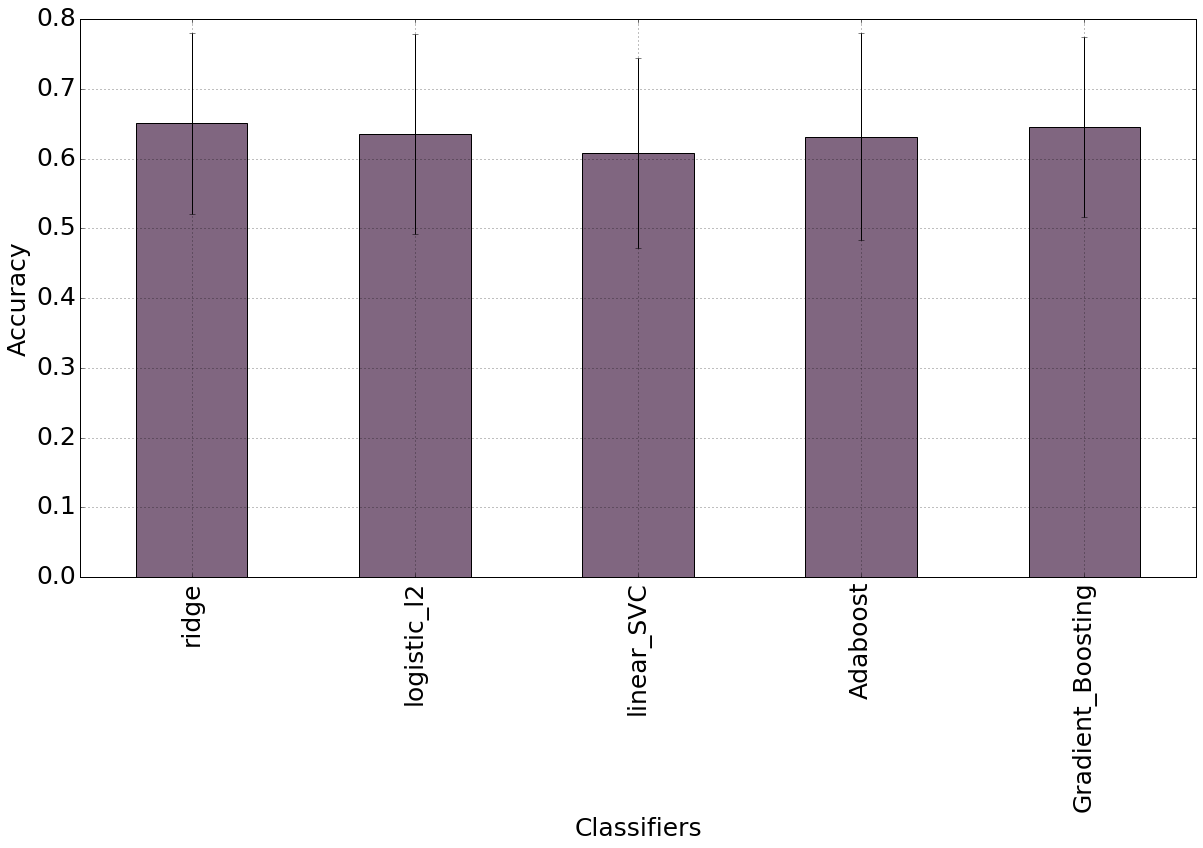
\includegraphics[width=0.9\textwidth]{barplot_index_classifiers}
    \caption{Condensed features approach results by classifier.}
    \label{fig:results2}
\end{figure}

In order to determine the feature importance in our models we ran 1000 loops of our training procedure for Ridge classifier and saved the feature coefficients for each round. Then we took the absolute value of the coefficients and summed over all iterations. The results of this is shown in table \ref{tab:feature_imp}. From this analysis we observe that the use of personal pronouns is the one that more information contains at the time of determining if a study is replicable or not. 

\begin{center}
\label{tab:feature_imp}
    \begin{tabular}{c|c}
        Feature     & Weight Score \\ \hline \hline
        i           & 1255.466658  \\ 
        we          & 1236.214745  \\ 
        they        & 1206.595188  \\ 
        shehe       & 1199.359474  \\ 
        you         & 1172.457431  \\
        ipron       &  637.496550  \\
        pronoun     &  634.866243  \\
        cause       &   32.348822  \\
        cogproc     &   30.105413  \\
    \end{tabular} \\

    Table \ref{tab:results_1}. Top 5 features in Ridge classifier.  
\end{center}

The full table with results can be found in Appendix B. 


\section{Conclusions}

Both sparse and condensed representations of text performed better than expected in almost all the splits we made. The results pointed out Naive Bayes as the best over all the models we trained. The mean accuracy for this model was around 68\%, which represents a statically significant improvement over a random decision.  After analyzing the most predictive words for each class, we realize that they do not have significant content, and thus we cannot make deeper conclusions about these results without access to further labeled data.  
The second approach also showed high predictive performance. If we contrast our results with the classifier developed by Markowitz, D. M. \& Hancock, J. T. \cite{prev2}, it can be seen an improvement in the mean accuracy for all the models we trained (63.2\% vs. 57.2\%). It is worth noticing that in this previous work they used a more than 400 observations dataset and their labels were more robust in the sense that the papers they declared unreplicable were actually retracted by their authors. This performance gain can be explained by the decision of ensemble all the feature indexes through machine learning and not just by the sum of some indices as in their approach.

Finally, our main conclusion of the project is that because of the lack of papers in the sample is difficult to test the robustness of the results, but our results show that there is space for further research in the field. A larger sample set would produce more stable models and probably easier to understand. However, this is a high level starting point to analyze the replicability of papers with text analysis and machine learning tools.   


\section{Future Work}

The work described in this paper has been concerned with the limited evidence of papers replicability. In this line, the next step would be definitely increase the sample of replicated and non replicated papers. We expect an enhance on the performance and higher generalization properties for the models. Further labeled data would also help us identify in which kind of papers each of the approaches works better and probably design a unique classifier with an overall best performance. This final classifier could be an improvement of one of the models already developed or probably an ensemble method of a classifier trained on condensed features representation and one trained on sparse features representation in order to extract as much information as possible from the text. 



% Your references go at the end of the main text, and before the
% figures.  For this document we've used BibTeX, the .bib file
% scibib.bib, and the .bst file Science.bst.  The package scicite.sty
% was included to format the reference numbers according to *Science*
% style.
\pagebreak
\bibliography{scibib}
%\bibliographystyle{Science}

\begin{thebibliography}{9}
\bibitem{nature1} Nature 525, 25–27 (03 September 2015), doi:10.1038/525025a
\bibitem{begley} Begley, C. G. Ellis, L. M. Nature 483, 531–533 (2012)
\bibitem{prinz} Prinz, F., Schlange, T.  Asadullah, K. Nature Rev. Drug Discov. 10, 712–713 (2011)
\bibitem{prev} Markowitz, D. M., \& Hancock, J. T. (2014). \emph{Linguistic traces of a scientific fraud: The case of Diederik Stapel}. PLoS ONE, 9, e105937
\bibitem{prev2} Markowitz, D. M., \& Hancock, J. T. (2015). \emph{Linguistic Obfuscation in Fraudulent Science}. Journal of Language and Social Psychology I–II. 2015 DOI: 10.1177/0261927X15614605.
\bibitem{rep_proj} Open Science Collaboration. (2015). \emph{Estimating the reproducibility of psychological science}. Science, 349(6251), aac4716. doi: 10.1126/science.aac4716.
\bibitem{pdfx} Constantin, Alexandru and Pettifer, Steve and Voronkov, Andrei. \emph{PDFX: Fully-automated PDF-to-XML Conversion of Scientific Literature}. Proceedings of the 2013 ACM Symposium on Document Engineering (2013). doi: 10.1145/2494266.2494271.
\bibitem{LIWC1} Yla R. Tausczik1, James W. Pennebaker1. \emph{The Psychological Meaning of Words: LIWC and Computerized Text Analysis Methods}. Journal of Language and Social Psychology. 29(1) 24–54. 2010 SAGE Publications. doi: 10.1177/261927X09351676.
\bibitem{LIWC2} Pennebaker, J.W., Boyd, R.L., Jordan, K., \& Blackburn, K. (2015). The development and psychometric properties of LIWC2015. Austin, TX: University of Texas at Austin.




\end{thebibliography}
% Following is a new environment, {scilastnote}, that's defined in the
% preamble and that allows authors to add a reference at the end of the
% list that's not signaled in the text; such references are used in
% *Science* for acknowledgments of funding, help, etc.
\pagebreak

\section*{Appendix A: LIWC Categories explained}
\label{appa}
\begin{itemize}
  \item Analytic: analytical thinking.
  \item Clout.
  \item Authentic. 
  \item Tone: emotional tone of the text. 
  \item WPS: words per sentence
  \item Sixltr: words with more than 6 letters. 
  \item Dic: dictionary words. The lower these value the higher the jargon use in the text. 
  \item function: function words (it, to, no very)
  \item pronoun (subset of function): pronouns (I, them, itself)
  \item ppron (subset of pronoun): Personal pronouns (I, them, her )
  \item i (subset of ppron): 1st pers singular (I, me, mine)
  \item we (subset of ppron): 1st pers plural (we, us, our)
  \item you (subset of ppron): 2nd person (you, your, thou )
  \item shehe (subset of ppron): 3rd pers singular (she, her, him)
  \item they (subset of ppron): 3rd pers plural (they, their, they’d )
  \item ipron (subset of pronoun): Impersonal pronouns (it, it’s, those )
  \item prep (subset of function): Prepositions (am, will, have)
  \item adverb (subset of function): Common Adverbs (very, really) 
  \item conj (subset of function): Conjunctions (and, but, whereas)
  \item negate (subset of function): Negations (no, not, never )
  \item compare: Comparisons (greater, best, after)
  \item number: Numbers (second, thousand)
  \item quant: Quantifiers (few, many, much )
  \item cogproc: Cognitive processes (cause, know, ought)
  \item insight (subset of cogproc): Insight (think, know)
  \item cause (subset of cogproc): Causation (because, effect)
  \item discrep (subset of cogproc): Discrepancy (should, would )
  \item tentat (subset of cogproc): Tentative (maybe, perhaps)
  \item certain (subset of cogproc): Certainty (always, never)
  \item differ (subset of cogproc): Differentiation (hasn’t, but, else)
\end{itemize}


\section*{Appendix B: Classifier's Results}
\label{appb}

\centering
\label{my-label}
\begin{tabular}{|l|l|l|}
\hline
Classifier          & Mean Accuracy & Standard Deviation \\ \hline \hline
Naive Bayes         & \textbf{0.68}          & 0.13               \\ \hline
SVM (TFIDF)         & 0.65          & 0.13               \\ \hline
SVM (DFM)           & 0.62          & 0.14               \\ \hline
Ridge               & 0.64          & 0.14               \\ \hline
Logistic Regression & 0.64          & 0.13               \\ \hline
Linear SVM          & 0.59          & 0.15               \\ \hline
Adaboost            & 0.64          & 0.14               \\ \hline
Gradient Boosting   & \textbf{0.65}          & 0.13               \\ \hline
\end{tabular}
% For your review copy (i.e., the file you initially send in for
% evaluation), you can use the {figure} environment and the
% \includegraphics command to stream your figures into the text, placing
% all figures at the end.  For the final, revised manuscript for
% acceptance and production, however, PostScript or other graphics
% should not be streamed into your compliled file.  Instead, set
% captions as simple paragraphs (with a \noindent tag), setting them
% off from the rest of the text with a \clearpage as shown  below, and
% submit figures as separate files according to the Art Department's
% instructions.


%\clearpage




\end{document}




















